% \documentclass[12pt]{article}

%%v helpful MIT exam schema, see http://www-math.mit.edu/~psh/exam/examdoc.pdf
 \documentclass[8pt]{exam} 
% \qformat{\textbf{Question \thequestion}\quad \thepoints\hfill } % Large depth to make space}
 \renewcommand{\thesubpart}{(\roman{subpart})}
 \renewcommand{\subpartlabel}{\thesubpart}
 \footer{}{}{Page \thepage\ de \numpages}
\addpoints
% \pointsinmargin
% \boxedpoints
\renewcommand{\questionshook}{\setlength{\itemsep}{0.2cm}}
\renewcommand{\partshook}{
	\setlength{\itemsep}{0.1cm}
}

\usepackage{cmbright}

\pagestyle{empty} %for handouts
% \addtolength{\jot}{2em} % this makes all formulae a bit more spaced vertically for handouts
\setlength{\parindent}{0pt} %we're not writing a novel
%\renewcommand{\arraystretch}{2} %makes tables taller, so easier to write in

\usepackage[fleqn]{amsmath}
\usepackage{amssymb} %standard classy maths symbols
\usepackage[a4paper, margin=1in]{geometry} %makes it easy to specify where to put stuff on the page

\usepackage{siunitx} %v handy way of getting SI units to typeset correctly...
% \sisetup{locale = FR} %... and now it will use a comma for decimals

\usepackage[utf8]{inputenc}

% \usepackage[french]{babel} % frenchify everything (e.g. a Table becomes a Tableau)
% \usepackage{lmodern} % font with nicer French characters than standard
% \usepackage{textcomp} % and more help for special characters

\usepackage{tcolorbox} % basic but good package for boxes around text
\tcbset{colback=black!5!white}
% \usepackage{color} % colours
%\newcommand{\fillin}{\color{black!1!white}} %makes the text disappear
%\definecolor{fillin}{rgb} {1.00,1.00,1.00}
%\renewcommand{\fillin}{\color{blue}} \definecolor{fillin}{rgb} {0.00,0.00,1.00} %makes the filling in text appear (in blue)

\usepackage{enumitem} % can change the labels on lists, items, enumerates
\usepackage{setspace}

\usepackage{tikz, pgfplots} % interval diagrams, sets, etc.
\usetikzlibrary{calc,trees,positioning,arrows,fit,shapes}

\begin{document}

\textbf{Name:} \dotfill

\

\begin{questions}

\question[1] In the story overleaf, how many grains of rice will there be on the last square? 
\fillwithdottedlines{7mm}

\question[3] Find a rule for the total number of grains of rice after $n$ squares.
\fillwithdottedlines{50mm}

\question[1] Find the total number of grains of rice on the chessboard.
\fillwithdottedlines{7mm}

\question[2] Follow the example below to calculate the weight of the rice on the chessboard in metric tonnes, given that a grain of rice weighs \SI{0,029}{g} and that there is $10^6$ grams in a metric tonne. \\
\textbf{Give your answer in scientific notation.}

\emph{If you are not sure of the total number of grains of rice, assume that there are $2^{50}$ grains in total.}

\

\begin{minipage}[c]{0.3\textwidth}
Example with 23 grains of rice:
\begin{align*}
&\mbox{23 grains of rice} \\
=& 23 \cdot 0,029 \,\, \mbox{g} \\
=& 23 \cdot 0,029 \cdot 10^{-6} \,\, \mbox{metric tonnes} \\
=& 6,67 \cdot 10^{-7} \,\, \mbox{metric tonnes}
\end{align*}

\end{minipage}
\vline
\hspace{2mm}
\begin{minipage}[c]{0.6\textwidth}
\vspace{-3mm}
\fillwithdottedlines{39mm}
\end{minipage}

\

\question[1] The current world production of rice is 495,87 million metric tonnes per year. So how many \textbf{years} would it take \textbf{the world} to fulfil the wish of rice on the chessboard?
\fillwithdottedlines{35mm}


\end{questions}




\vfill

\begin{tcolorbox}

\textbf{Name of examiner:}

\begin{center}
\gradetable[h][questions]
\end{center}

\end{tcolorbox}

\newpage

Please read the following story, answer the question below, then wait for permission to turn over.

\

{\bfseries Question: Do you think you could lift the chessboard once the rice is in place?}

\vspace{1cm}

\begin{center}
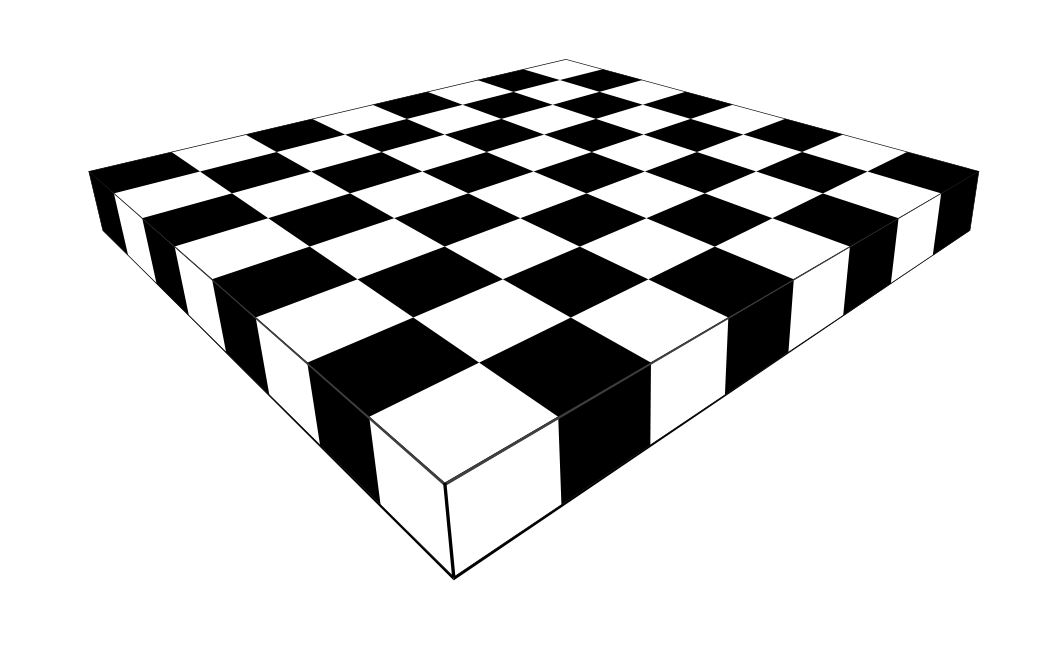
\includegraphics{chessboard.jpg}
\end{center}

\vspace{1cm}

\begin{tcolorbox}[left skip=10mm, right skip=10mm]
There's a famous legend about the origin of chess that goes like this. When the inventor of the game showed it to the emperor of India, the emperor was so impressed by the new game, that he said to the man

\begin{center}
\emph{``Name your reward!"}
\end{center}

The man responded,

\begin{center}
\emph{``Oh emperor, my wishes are simple. I only wish for this. Give me one grain of rice for the first square of the chessboard, two grains for the next square, four for the next, eight for the next and so on for all 64 squares, with each square having double the number of grains as the square before."}
\end{center}

\

The emperor agreed, amazed that the man had asked for such a small reward - or so he thought...
\end{tcolorbox}




\end{document}